\documentclass[a4paper,12pt,oneside]{article}
\usepackage[utf8]{inputenc}
\usepackage[polish]{babel}
\usepackage[T1]{fontenc}
\usepackage{graphicx}
\usepackage{enumitem}
\usepackage{pdfpages}

\begin{document}
	\begin{titlepage}
		\begin{center}
			
\includegraphics[keepaspectratio]{agh.jpg}\\[0.5cm]
			{\large Wydział Elektrotechniki, Automatyki, Informatyki \\i~Inżynierii Biomedycznej}\\[0.5cm]
			{\huge Projekt założenia spółki z ograniczoną odpowiedzialnością}\\[1cm]
			\begin{table}[!h]
				\begin{tabular}{ll}
					Kierunek: & Informatyka \\
					Przedmiot: & Aspekty prawne i organizacja przedsiębiorstwa\\
					Prowadzący: & dr inż. Marta Kraszewska\\
					Autorzy: &Banaś Sebastian\\
					&Bogacz Marcin\\
					&Królikowski Michał\\
					&Michałkiewicz Krzysztof\\
				\end{tabular}
			\end{table}
		\end{center}
	\end{titlepage}

	\tableofcontents
	
	\section{Informacje wstępne}
\subsection{Cel i okoliczności powstania}
Jesteśmy grupą studentów informatyki, więc zrozumiałe jest, że jesteśmy zafascynowani wszelkimi nowościami technologicznymi. Podczas jednego z naszych spotkań powstał pomysł, aby założyć firmę zajmującą się sprowadzaniem oraz sprzedażą najnowszych nowinek technologicznych od naszych przyjaciół z dalekiego wschodu. Naszym celem jest stworzenie przedsiębiorstwa, które uprości i przyspieszy zakupy chińskich produktów. W tej chwili bardzo dużo osób dokonuje takich zakupów na własną rękę martwiąc się o to kiedy lub czy w ogóle przesyłka dotrze albo zastanawiając się czy wygenerowane zostaną dodatkowe koszty dzięki wizycie w Urzędzie Celnym. Chcemy z tym skończyć. Nasza firma będzie sprowadzać sprzęt z Chin w możliwie najkorzystniejszych cenach oraz wysyłać i serwisować sprzęt na terenie naszego kraju. Aby to osiągnąć utworzymy nasz sklep internetowy, który będzie stanowił główne źródło pozyskiwania klientów. Ponieważ jesteśmy bardzo zdolnymi i ambitnymi studentami, stworzenie takiego sklepu nie będzie stanowiło najmniejszego problemu.
\subsection{Działalność przedsiębiorstwa}
Naszą główną działalnością będzie sprowadzanie, sprzedaż oraz serwis urządzeń elektronicznych z Chińskiej Republiki Ludowej. Obszarem, na którym będziemy działać jest terytorium naszego kraju. Docelową grupą klientów, którą będziemy chcieli pozyskać są młodzi ludzi, którzy zainteresowani są zakupem niekoniecznie markowych urządzeń, za to koniecznie w najniższej cenie. Naszą działalność chcemy promować głównie poprzez aktywne prowadzenie profili na portalach społecznościowych.
\subsection{Forma prawna}
Formą prawną, która została przez nas przyjęta jest spółka z ograniczoną odpowiedzialnością. W Polsce jest to druga najczęściej wybierana forma działalności gospodarczej. Może ona zostać utworzona przez jedną lub więcej osób, które nazywane są wspólnikami. Wspólnikami mogą być również inne podmioty posiadające osobowość prawną z jednym wyjątkiem. Jednoosobową spółkę z ograniczoną odpowiedzialnością nie może założyć inna jednoosobowa spółka z ograniczoną odpowiedzialnością. 

W Polsce spółka z o.o. jest spółką handlową regulowaną przez Kodeks spółek handlowych. Wspólnicy nie odpowiadają własnym majątkiem za zobowiązania wobec wierzycieli powstałe w wyniku prowadzonej działalności. Spółka odpowiada za nie całym swoim majątkiem. Jedynie w przypadku nieskutecznej egzekucji należności, członkowie zarządu mogą solidarnie odpowiadać za zobowiązania własnym majątkiem. Aby tego uniknąć członek zarządu powinien wykazać, że w odpowiednim momencie złożył wniosek o ogłoszenie upadłości. 

Do założenia spółki z ograniczoną odpowiedzialnością wymagana jest umowa w postaci aktu notarialnego. Można ją zastąpić umową w postaci elektronicznej podpisanej podpisem elektronicznym przez każdego ze wspólników. Minimalny kapitał zakładowy wynosi 5000 zł. Wartość nominalna udziału nie może być niższa niż 50 zł. Spółka jest również zobowiązana do prowadzenia ksiąg rachunkowych.

Organy spółki z ograniczoną odpowiedzialnością:
\begin{itemize}
	\item Zgromadzenie wspólników - najwyższa władza spółki. Podejmuje uchwały większością głosów. 
	\item Zarząd - powoływany jest przez zgromadzenie wspólników. Minimalnie jest to jedna osoba. Zarząd reprezentuje oraz prowadzi sprawy spółki. 
	\item Rada nadzorcza - jest obligatoryjna tylko w dwóch przypadkach: kapitał zakładowy osiągnął 500 000 zł i liczba wspólników jest większa od 25 osób lub spółka powstała ze spółki Skarbu Państwa. Zadaniem rady nadzorczej jest nadzór nad działalnością we wszystkich dziedzinach.
\end{itemize}

\subsection{Postępowanie przygotowawcze w celu założenia przedsiębiorstwa}
Przed przystąpieniem do kompletowania dokumentów niezbędnych do założenia działalności ustaliliśmy początkowe założenia. Wspólnikami w spółce będą: Sebastian Banaś, Marcin Bogacz, Michał Królikowski oraz Krzysztof Michałkiewicz. Jednocześnie ten sam skład osobowy będzie stanowił zarząd.

Nazwą naszej firmy będzie: ChinaElectronics Spółka z o.o. z siedzibą: ul. Rozrywka 1, 30-001 Kraków. Ustaliliśmy również, że kapitał zakładowy będzie wynosił 5000 zł, a wartość nominalna udziału będzie wynosić 1250zł. Każdy ze wspólników będzie posiadał jeden udział w spółce. Czas trwania spółki ustalamy jako nieograniczony.

W tym samym czasie udało nam się znaleźć dogodną lokalizację dla naszej działalności. Odbyliśmy wstępne rozmowy dotyczące wynajmu lokalu. Każdy ze wspólników zobowiązał się również do czasowego udostępnienia własnego sprzętu komputerowego na cele prowadzenia działalności spółki. %Jednocześnie wszyscy solidarnie będą ponosić koszty rejestracji przedsiębiorstwa.
	\section{Rejestracja Firmy}
wymienić w punktach i krótko opisać (w odpowiedniej kolejności) instytucje do których należy się udać, aby móc rozpocząć własną działalność gospodarczą (notariusz, urząd gminy, Krajowy Rejestr Sądowy, Urząd Statystyczny, Urząd Skarbowy, bank, ZUS etc.)\\
jakie druki należy wypełnić w poszczególnych instytucjach?\\
jakie dokumenty należy posiadać?\\
wypełnić konieczne formularze i druki (wzory można ściągnąć internetu lub udać się do urzędu)\\
	\section{Formy opodatkowania przedsiębiorstwa}
\subsection{Dopuszczalne formy opodatkowania}
jakie są dopuszczalne formy opodatkowania Państwa 
przedsiębiorstwa?
\subsection{Wybrana forma opodatkowania}
jaką formę opodatkowania Państwo wybrali (krótka 
charakterystyka) i dlaczego?
	\section{Zatrudnianie pracowników}
\subsection{Procedura zatrudniania pracownika}
procedura zatrudniania pracownika (wymagane dokumenty i czynności)
\subsection{Zawarcie umowy}
zawarcie umowy o dzieło (KUP 50\%), umowy zlecenie, umowyo pracę
	\section{Wnioski}
jakie są zalety i wady formy prawnej Państwa przedsiębiorstwa?\\
jakie trudności (udogodnienia) napotkali Państwo w trakcie rejestracji firmy?\\
co Państwa zdaniem przyspieszyłoby proces rejestracji firmy?\\
inne nasuwające się wnioski\\
	
	Załączniki:
	\begin{enumerate}[label=Załącznik \arabic*]
		\item Akt notarialny
		\item Wniosek o rejestrację spółki z ograniczoną odpowiedzialnością (KRS-W3) 
	\end{enumerate}
	
	\centerline{\huge\textbf{AKT NOTARIALNY}}
\bigskip
Dnia 13.12.2017 r  ( dnia trzynastego grudnia dwa tysiące siedemnastego roku ) w Kancelarii Notarialnej w Krakowie stawili się :\\ \\
\textbf{Sebastian Banaś} syn Sebastiana zam. ul. Rozrywka 1, 30-001 Kraków PESEL 95010100001 legitymujący się dowodem osobistym seria ABC123456,\\ \\
\textbf{Marcin Bogacz} syn Marcina zam. ul. Rozrywka 1, 30-001 Kraków PESEL 95010100002 legitymujący się dowodem osobistym seria BBC123456,\\ \\
\textbf{Michał Królikowski} syn Michała zam. ul. Rozrywka 1, 30-001 Kraków PESEL 95010100003 legitymujący się dowodem osobistym seria CBC123456,\\ \\
\textbf{Krzysztof Michałkiewicz} syn Krzysztofa zam. ul. Rozrywka 1, 30-001 Kraków PESEL 95010100004 legitymujący się dowodem osobistym seria DBC123456,\\

\centerline{\large\textbf{UMOWA SPÓŁKI Z OGRANICZONĄ ODPOWIEDZIALNOŚCIĄ}}


\centerline{\large\textbf{POSTANOWIENIA OGÓLNE}}


\centerline{\large\textbf{§ 1}}

1. Stawiający oświadczają, że w celu prowadzenia działalności gospodarczej, zawiązują niniejszym spółkę z ograniczoną odpowiedzialnością, zwaną dalej Spółką.

2. Spółka będzie prowadzoną pod firmą "China Electronics spółka z ograniczoną odpowiedzialnością". Spółka może posługiwać się skrótem firmy China Electronics sp. zo.o., jego odpowiednikami w  językach obcych oraz wyróżniającym ją znakiem graficzny.

3. Siedzibą Spółki jest ul. Rozrywka 1, 30-001 Kraków.

4. Spółka działa na obszarze Rzeczypospolitej Polskiej i za granicą.\\

\centerline{\large\textbf{II. PRZEDMIOT DZIAŁALNOŚCI SPÓŁKI}}


\centerline{\large\textbf{§ 2}}

Przedmiotem działalności Spółki zgodnie z Polską Klasyfikacją Działalności (PKD) jest:

1) Sprzedaż hurtowa komputerów, urządzeń peryferyjnych i oprogramowania (PKD 46.51.Z);

2) Sprzedaż detaliczna komputerów, urządzeń peryferyjnych i oprogramowania prowadzona w wyspecjalizowanych sklepach (PKD 47.41.Z);

3) Działalność wydawnicza w zakresie pozostałego oprogramowania (PKD 58.29.Z);
\\

\centerline{\large\textbf{III. KAPITAŁ SPÓŁKI}}

\centerline{\large\textbf{§ 3}}

1. Kapitał zakładowy Spółki wynosi 50.000 zł ( pięćdziesiąt tysięcy złotych) i dzieli się na  500 udziałów po 100 zł (sto złotych) każdy udział.\\

\centerline{\large\textbf{§ 4}}

1. Kapitał zakładowy Spółki może być podwyższony do kwoty 10000 zł w terminie do 31.12.2018. r.

2. Podwyższenie kapitału zakładowego w trybie określonym w ustępie 1 nie wymaga zmiany umowy spółki.

3. Uchwałę o podwyższeniu kapitału zakładowego oraz o sposobie objęcia podwyższonego kapitału podejmuje Zgromadzenie Wspólników.\\

\centerline{\large\textbf{§ 5}}

1.Udziały w Spółce są równe i niepodzielne. Każdy wspólnik może mieć więcej niż jeden udział.

2.Udziały w kapitale zakładowym objęte zostały w następujący sposób :

- Sebastian Banaś obejmuje 1 udział,  o wartości 1250 zł każdy, o łącznej wartości 1250 zł, pokrywając je gotówką,

- Marcin Bogacz obejmuje 1 udział,  o wartości 1250 zł każdy, o łącznej wartości 1250 zł, pokrywając je gotówką,

- Michał Królikowski obejmuje 1 udział,  o wartości 1250 zł każdy, o łącznej wartości 1250 zł, pokrywając je gotówką,

- Krzysztof Michałkiewicz obejmuje 1 udział,  o wartości 1250 zł każdy, o łącznej wartości 1250 zł, pokrywając je gotówką,
3. Udziały mogą być umorzone za zgodą wspólnika.\\

\centerline{\large\textbf{§ 6}}

1.      Wspólnicy są zobowiązani do wnoszenia dopłat, proporcjonalnie do posiadanych udziałów.

2.      Wysokość i terminy dopłat oznaczone zostaną w miarę potrzeby uchwałą Zgromadzenia Wspólników.

3.      Dopłaty mogą być zwrócone wspólnikom na mocy uchwały Zgromadzenia Wspólników pod warunkiem, że nie są potrzebne do pokrycia strat bilansowych Spółki.\\

\centerline{\large\textbf{IV. ORGANY SPÓŁKI}}


\centerline{\large\textbf{§ 7}}

Organami Spółki są:

1. Zarząd Spółki.

2. Zgromadzenie Wspólników.\\

\centerline{\large\textbf{A. Zarząd}}


\centerline{\large\textbf{§ 8}}

1. Zarząd Spółki składa się z jednej do pięciu osób

2. Kadencja Zarządu Spółki trwa 5 (pięć ) kolejnych lat.

3. Zarząd jest powoływany i odwoływany przez Zgromadzenie wspólników.
\\
\centerline{\large\textbf{§ 9}}

1. Zarząd jest zobowiązany zarządzać majątkiem i sprawami Spółki, oraz spełniać swoje obowiązki ze starannością wymaganą w obrocie gospodarczym przestrzegając przepisów prawa, postanowień umowy, uchwał powziętych przez Zgromadzenie Wspólników. Do zakresu działania Zarządu należą sprawy Spółki niezastrzeżone do właściwości Zgromadzenia Wspólników.

2. Zarząd reprezentuje Spółkę względem osób trzech.

3. Do pierwszego składu Zarządu zostali powołani : Sebastian Banaś, Marcin Bogacz, Michał Królikowski oraz Krzysztof Michałkiewicz. Powierza się Sebastianowi Banaś pełnienie funkcji Prezesa Zarządu. Kolejne Zarządy zostaną ustanowione uchwałą Zgromadzenia Wspólników

4. Do reprezentowania Spółki uprawniony jest każdy członek zarządu samodzielnie.

\centerline{\large\textbf{B. Zgromadzenie Wspólników}}


\centerline{\large\textbf{§ 10}}

1. Zgromadzenie Wspólników obraduje na posiedzeniach zwyczajnych lub nadzwyczajnych.

2. Zwyczajne Zgromadzenie Wspólników zwołuje Zarząd Spółki z własnej inicjatywy w ciągu sześciu miesięcy po upływie każdego roku obrotowego.

3. Nadzwyczajne Zgromadzenie Wspólników zwołuje Zarząd Spółki z własnej inicjatywy lub na wniosek wspólników reprezentujących, co najmniej jedną dziesiątą kapitału zakładowego.

4. Zwołanie nadzwyczajnego Zgromadzenia Wspólników na wniosek wspólników powinno nastąpić w ciągu dwóch tygodni od daty zgłoszenia wniosku.\\

\centerline{\large\textbf{§ 11}}

1. Zgromadzenie Wspólników może podejmować uchwały jedynie w sprawach objętych porządkiem obrad.

2. Porządek obrad ustala Zarząd Spółki.

3. Wspólnicy reprezentujący, co najmniej jedną dziesiątą kapitału zakładowego mogą żądać umieszczenia poszczególnych spraw w porządku obrad najbliższego Zgromadzenia Wspólników.\\

\centerline{\large\textbf{§ 12}}

Zgromadzenia Wspólników odbywają się w siedzibie Spółki.\\

\centerline{\large\textbf{§ 13}}

Na każdy udział przypada jeden głos. Głosowanie przez pełnomocnika jest dopuszczalne.\\

\centerline{\large\textbf{§ 14}}

1. Uchwały Zgromadzenia Wspólników zapadają bezwzględną większością głosów oddanych, o ile przepisy ustawy lub niniejsza umowa nie stanowią inaczej.

2. W przypadku przewidzianym w art. 246 § 1 Kodeksu spółek handlowych do uchwały
o rozwiązaniu Spółki wymagana jest większość 3/4 (trzech czwartych) głosów.

\centerline{\large\textbf{§ 15}}

Głosowanie jest jawne. Tajne głosowanie zarządza się przy wyborach organów Spółki oraz nad wnioskami o odwołanie członków organów lub likwidatora Spółki, bądź  o pociągnięcie ich do odpowiedzialności, jak również w sprawach osobistych. Ponadto tajne głosowanie zarządza się na wniosek choćby jednego z obecnych uprawnionych do głosowania.\\

\centerline{\large\textbf{§ 16}}

1.      Zgromadzenie Wspólników otwiera Prezes Zarządu lub osoba przez niego wskazana, po czym spośród osób uprawnionych do głosowania wybiera się przewodniczącego Zgromadzenia.

2.      Zgromadzenie Wspólników uchwala swój regulamin określający szczegółowo tryb prowadzenia obrad\\

\centerline{\large\textbf{§ 17}}

1. Do wyłącznej kompetencji Zgromadzenia Wspólników należy:

1) rozpatrzenie i zatwierdzenie sprawozdania Zarządu z działalności Spółki oraz sprawozdania finansowego za ubiegły rok obrotowy;

2) powzięcie uchwały o podziale zysku lub sposobie pokrycia strat;

3) udzielenie absolutorium członkom organów Spółki z wykonania przez nich obowiązków;

4) zmiana przedmiotu działalności Spółki;

5) zmiana umowy Spółki;

6) połączenie, przekształcenie i utworzenie nowej Spółki lub przystąpienie do innej Spółki;

7) podwyższenie lub obniżenie kapitału zakładowego;

8) wyrażenie zgody na obciążenie udziałów lub ustanowienie na nich zastawu oraz na zbycie udziałów, także na rzecz Spółki w celu ich umorzenia;

9) umorzenie udziałów;

10) powzięcie uchwały o wysokości i terminie dopłat oraz ich ewentualnym zwrocie;

11) rozwiązanie i likwidacja Spółki;

12) zbycie i wydzierżawienie przedsiębiorstwa Spółki lub jego zorganizowanej części oraz ustanowienie na nich ograniczonego prawa rzeczowego;

13) postanowienie co do dalszego istnienia Spółki w przypadku, gdy straty przekraczają sumę funduszu zapasowego i połowę kapitału zakładowego;

14) ustalenie wynagrodzenia dla  Zarządu Spółki;

15) postanowienie dotyczące roszczeń o naprawienie szkody wyrządzonej przy sprawowaniu zarządu .

2. Oprócz spraw wymienionych w ustępie 1. uchwały Zgromadzenia Wspólników wymagają sprawy określone w innych postanowieniach niniejszej umowy oraz w Kodeksie spółek handlowych.

3. Nabycie i zbycie nieruchomości, użytkowania wieczystego lub udziału w nieruchomości nie wymaga uchwały Zgromadzenia Wspólników.\\

\centerline{\large\textbf{V. GOSPODARKA SPÓŁKI}}

\centerline{\large\textbf{§ 18}}

Organizację Spółki określa regulamin organizacyjny ustalony przez Zarząd Spółki.\\

\centerline{\large\textbf{§ 19}}

1. Spółka prowadzi rachunkowość zgodnie z obowiązującymi przepisami.

2. Rokiem obrotowym Spółki jest rok kalendarzowy, za wyjątkiem pierwszego roku obrotowego, który kończy się 31.12.2018 r .\\

\centerline{\large\textbf{§ 20}}

Zarząd Spółki jest zobowiązany przedłożyć na piśmie Zgromadzeniu Wspólników roczne sprawozdanie finansowe oraz roczne sprawozdanie z działalności Zarządu Spółki, w czasie umożliwiającym odbycie zwyczajnego Zgromadzenia Wspólników bez naruszania terminu określonego w przepisach powszechnie obowiązujących.\\

\centerline{\large\textbf{§ 21}}

1. Czysty zysk wynikający z rocznego bilansu przeznaczony jest na kapitał zapasowy, o ile wspólnicy nie rozporządzą inaczej.

2. Wspólnicy mogą przeznaczyć zysk lub jego część do podziału między siebie oraz przeznaczyć na fundusz zapasowy lub inne fundusze określone w uchwale Zgromadzenia Wspólników.

3. Zysk lub jego część przeznaczoną uchwałą Zgromadzenia Wspólników do podziału między wspólników dzieli się w stosunku proporcjonalnym do udziałów wspólników.\\

\centerline{\large\textbf{VI. POSTANOWIENIA KOŃCOWE}}

\centerline{\large\textbf{§ 22}}

1. Spółka zamieszcza wymagane prawem ogłoszenia w "Monitorze Sądowym i Gospodarczym".\\

\centerline{\large\textbf{§ 23}}

Koszty tego aktu ponosi Spółka.

	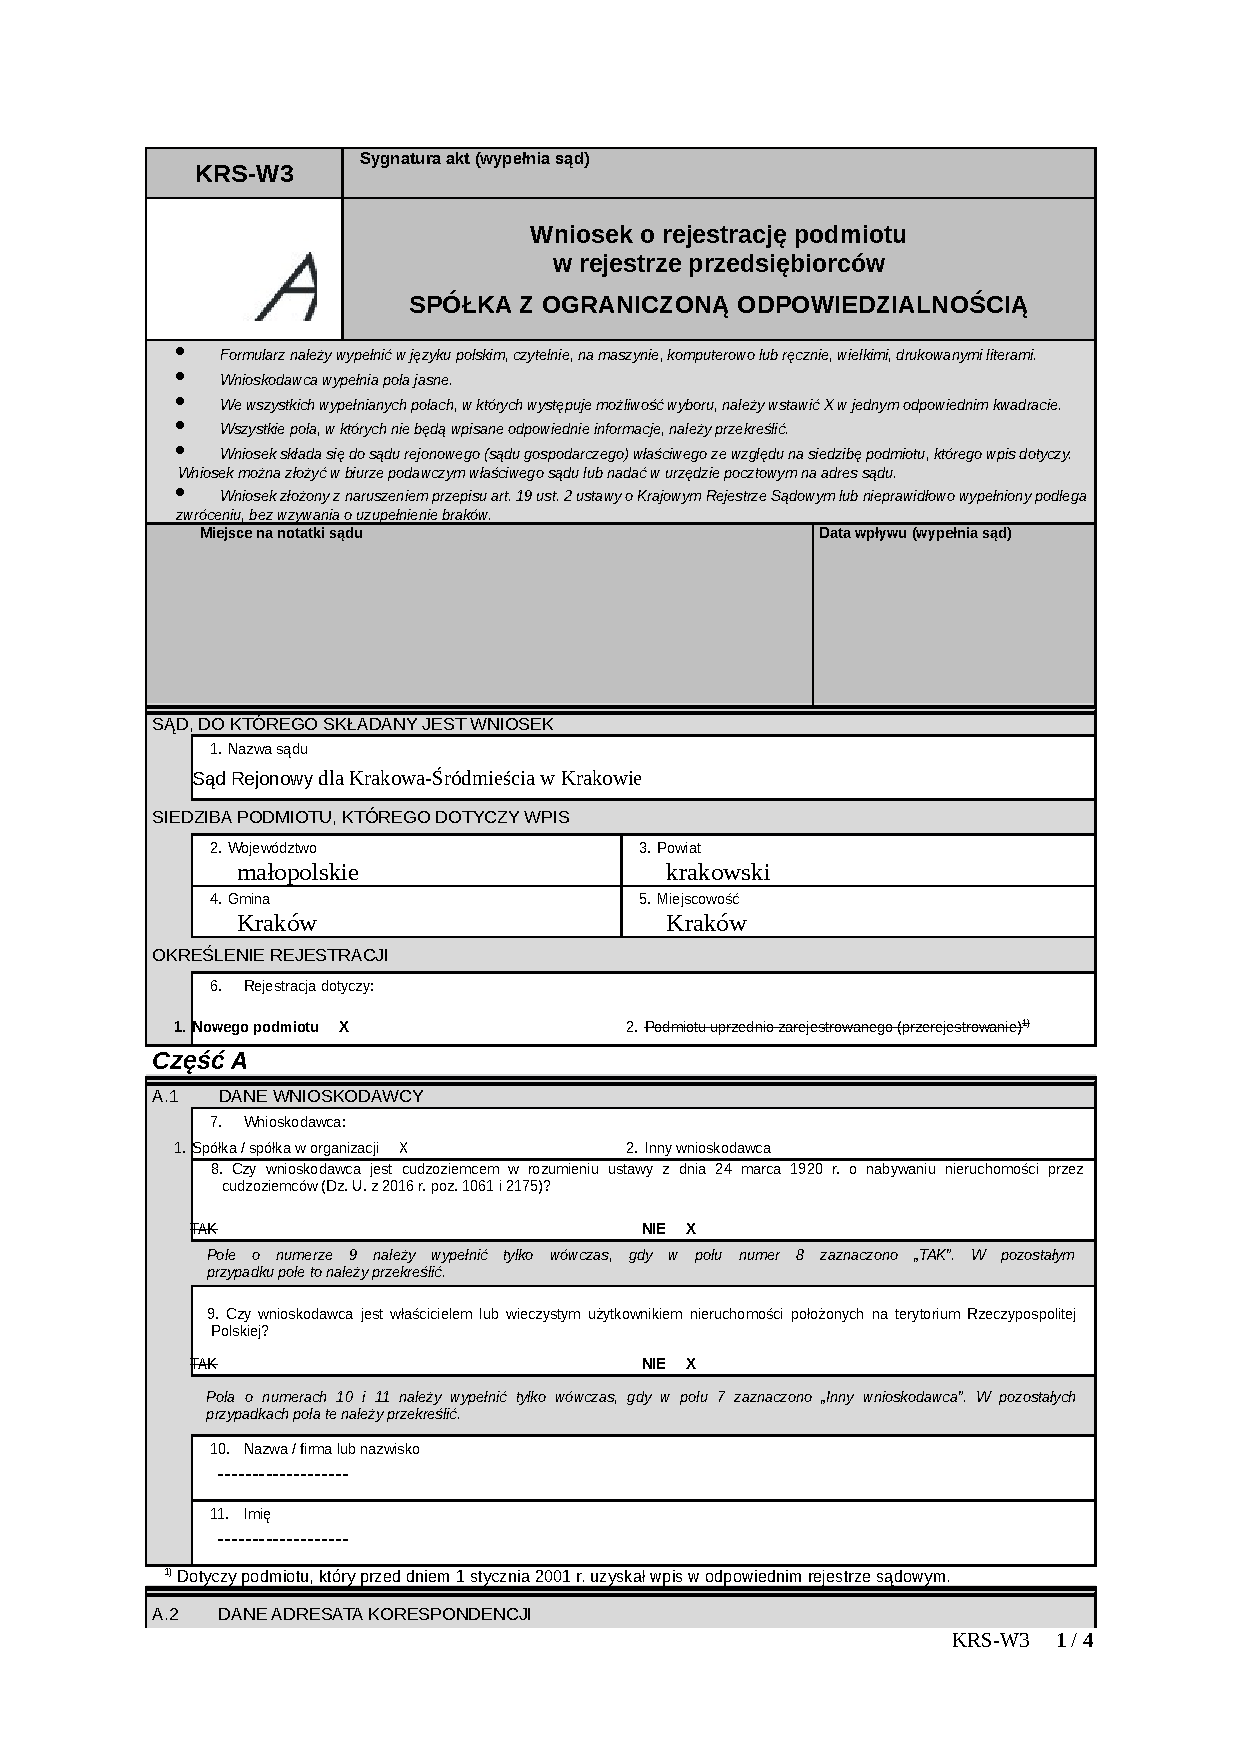
\includepdf[page=-]{zalaczniki/krs-w3.pdf}
\end{document}